\chapter{Experiements}
%\section{Experiments}

\section{Training sets}
\prettyref{sec:learnForTheTask} mentions that one of the key
elements of the learning algorithms is the learning of specialization
dictionaries. Task specific training data is a common way to solve the problem
of finding  the right dictionary. Here learning for the task comes into
account. Such as de-noising or in-painting dictionaries directly learned from
the initial signal that gets de-noised or restored from in-painting. If the task
gets bigger it sounds logical to increase the size of training data and take a
bigger variety of signals to learn from.  We use da database of 100,000
to 1,000,000 natural JPEG images collected from \url{flickr.com}. And we have a
closer look at differences of learned elements from a smaller specific set of
sketch images in PNG format. (\prettyref{fig:database_images})
%via clustered training with a large image
% These sets include sketches, still images of animations from Disney and
% post-impressionistic images from Vincent van Gogh.  

\begin{figure}[h]
\centering
% \subfloat{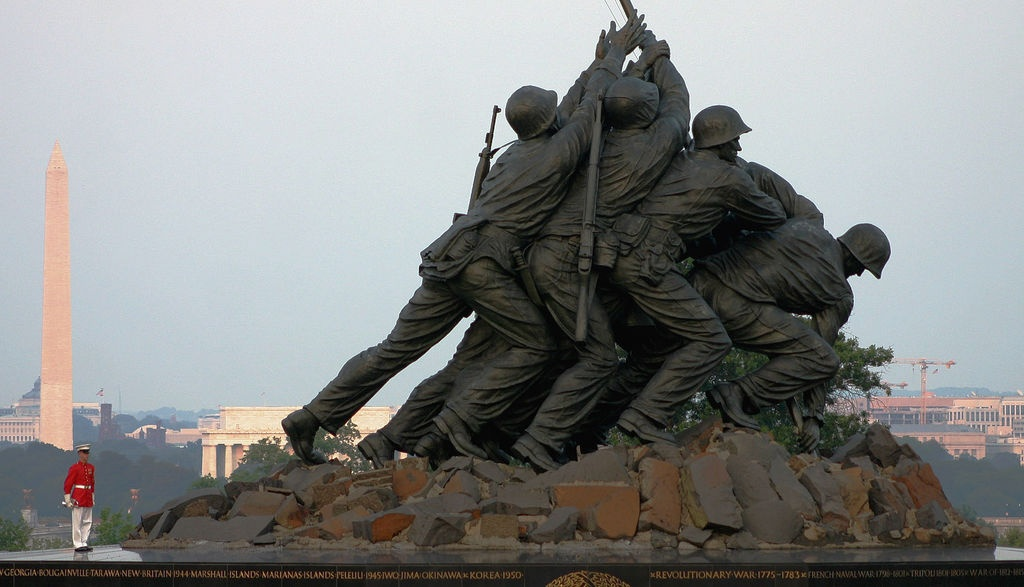
\includegraphics[width = 0.3\textwidth]{images/28979823.jpg}}
% \hspace{5mm}
% \subfloat{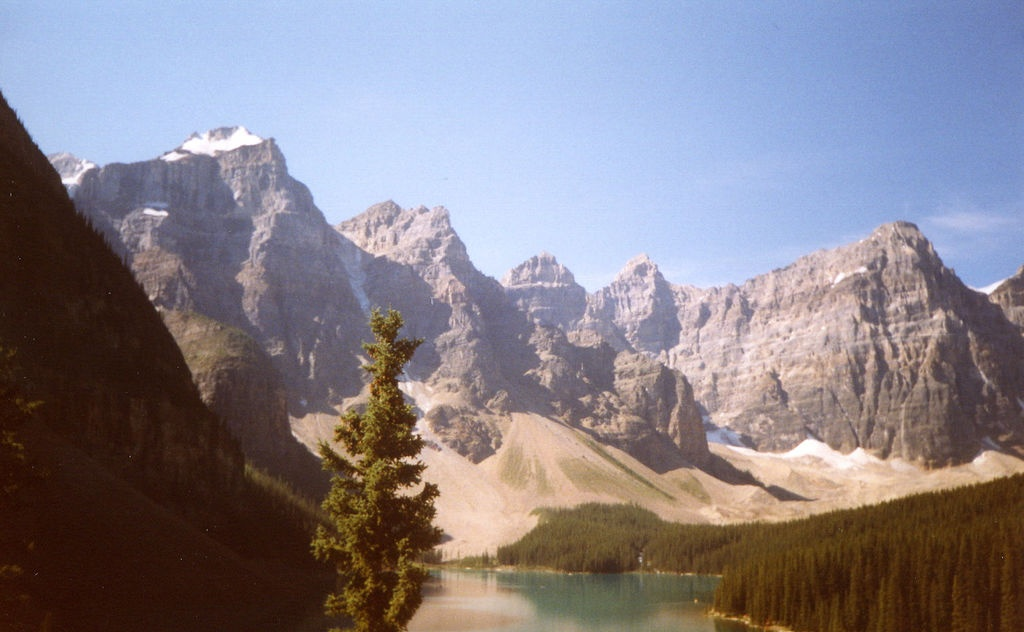
\includegraphics[width = 0.3\textwidth]{images/29018694.jpg}}
% \hspace{5mm}
% \subfloat{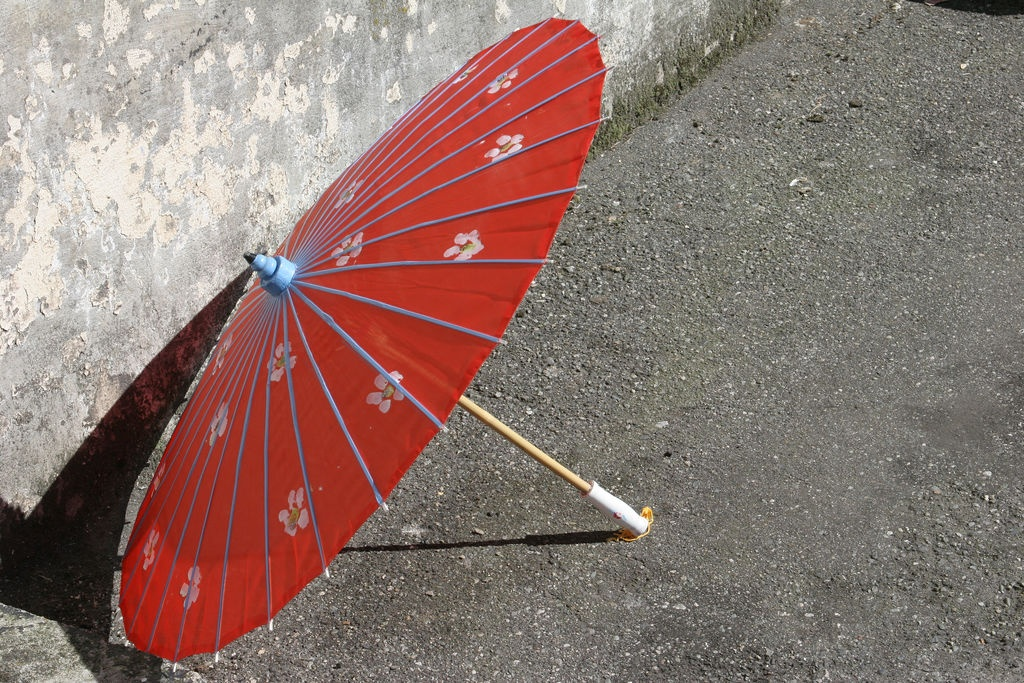
\includegraphics[width = 0.3\textwidth]{images/28874882.jpg}}
% \hspace{5mm}
\subfloat{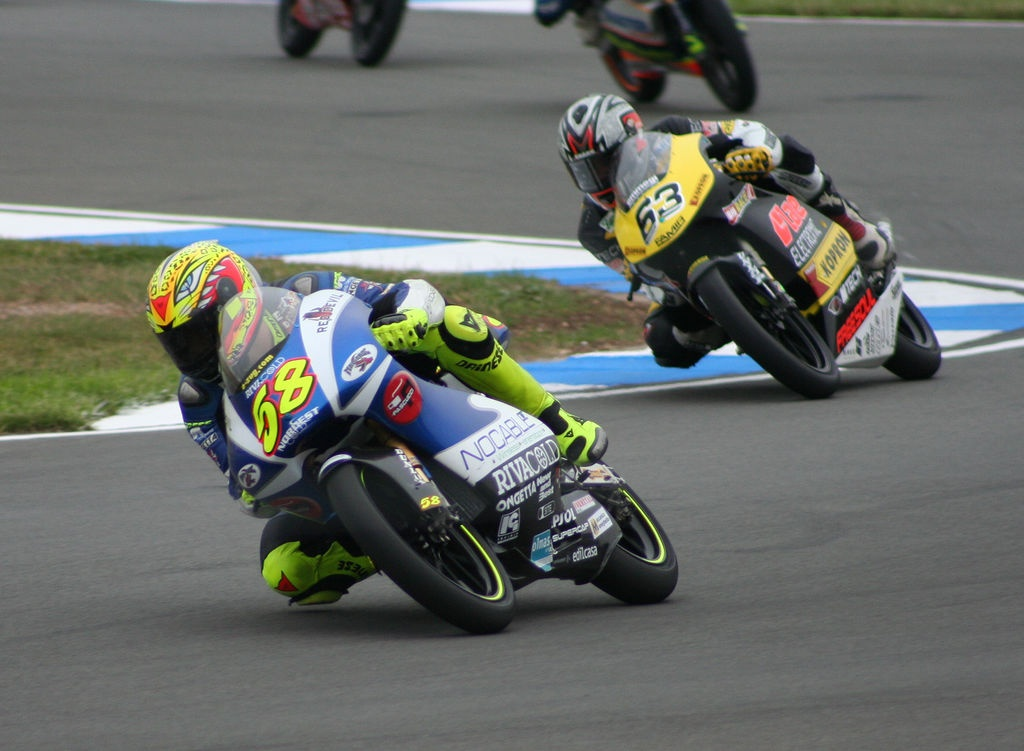
\includegraphics[width = 0.3\textwidth]{images/28803842.jpg}}
\hspace{5mm}
\subfloat{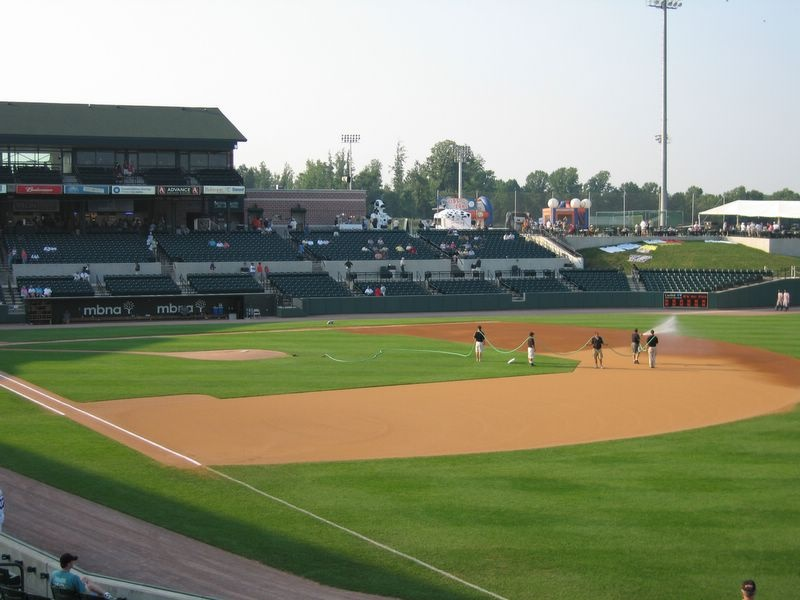
\includegraphics[width = 0.3\textwidth]{images/28894495.jpg}}
\hspace{5mm}
\subfloat{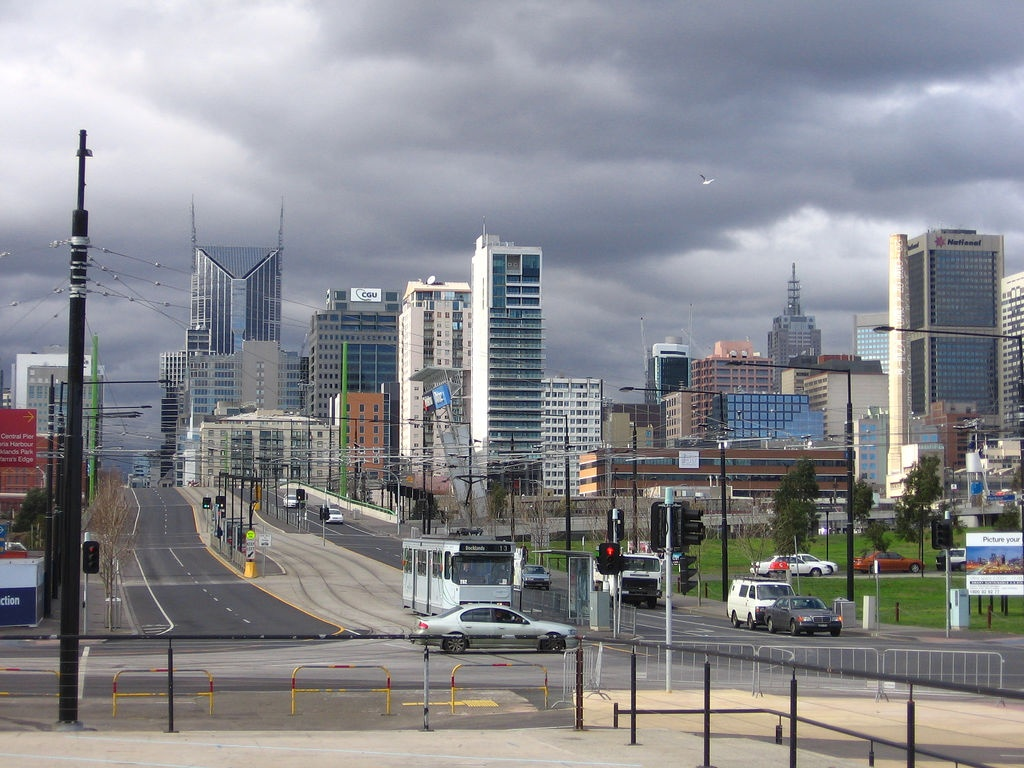
\includegraphics[width = 0.3\textwidth]{images/28952841.jpg}}
\hspace{5mm}
\subfloat{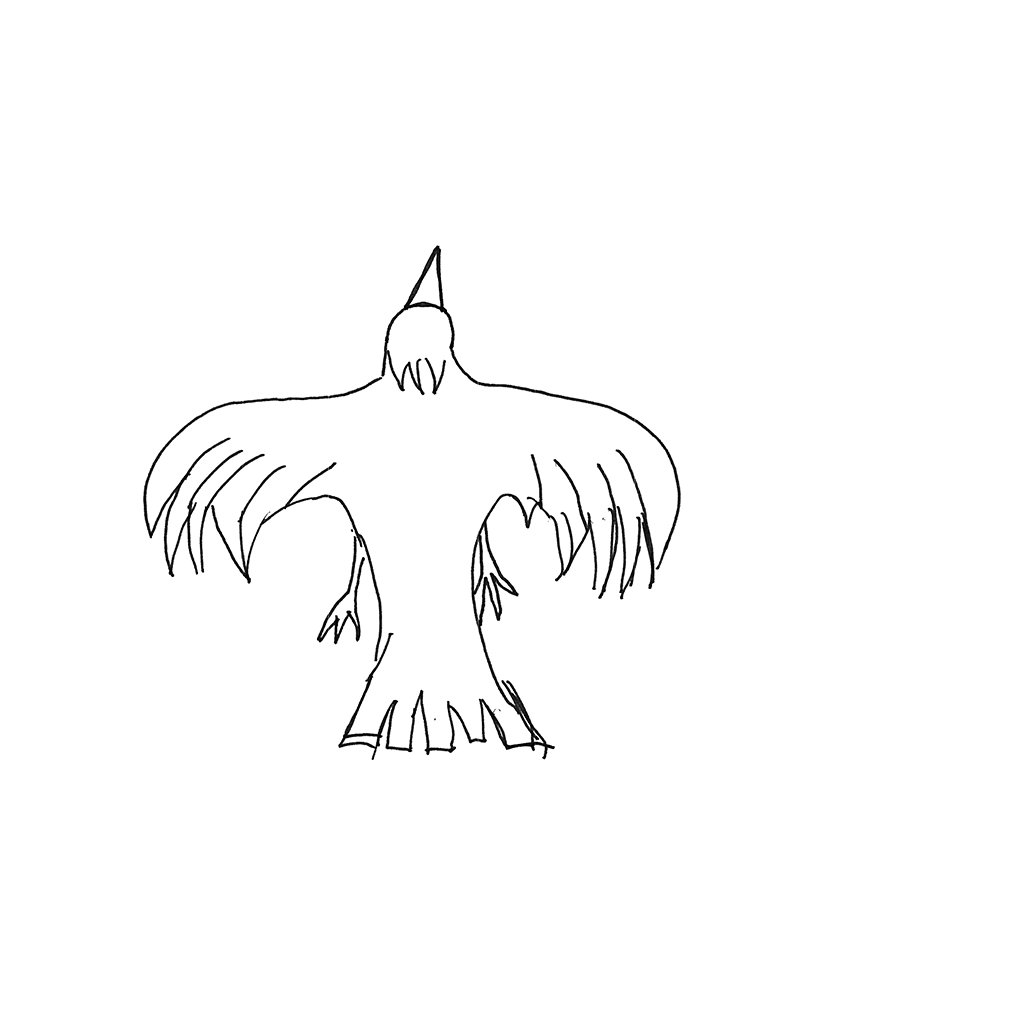
\includegraphics[width = 0.3\textwidth]{images/sketch1.jpg}}
\hspace{5mm}
\subfloat{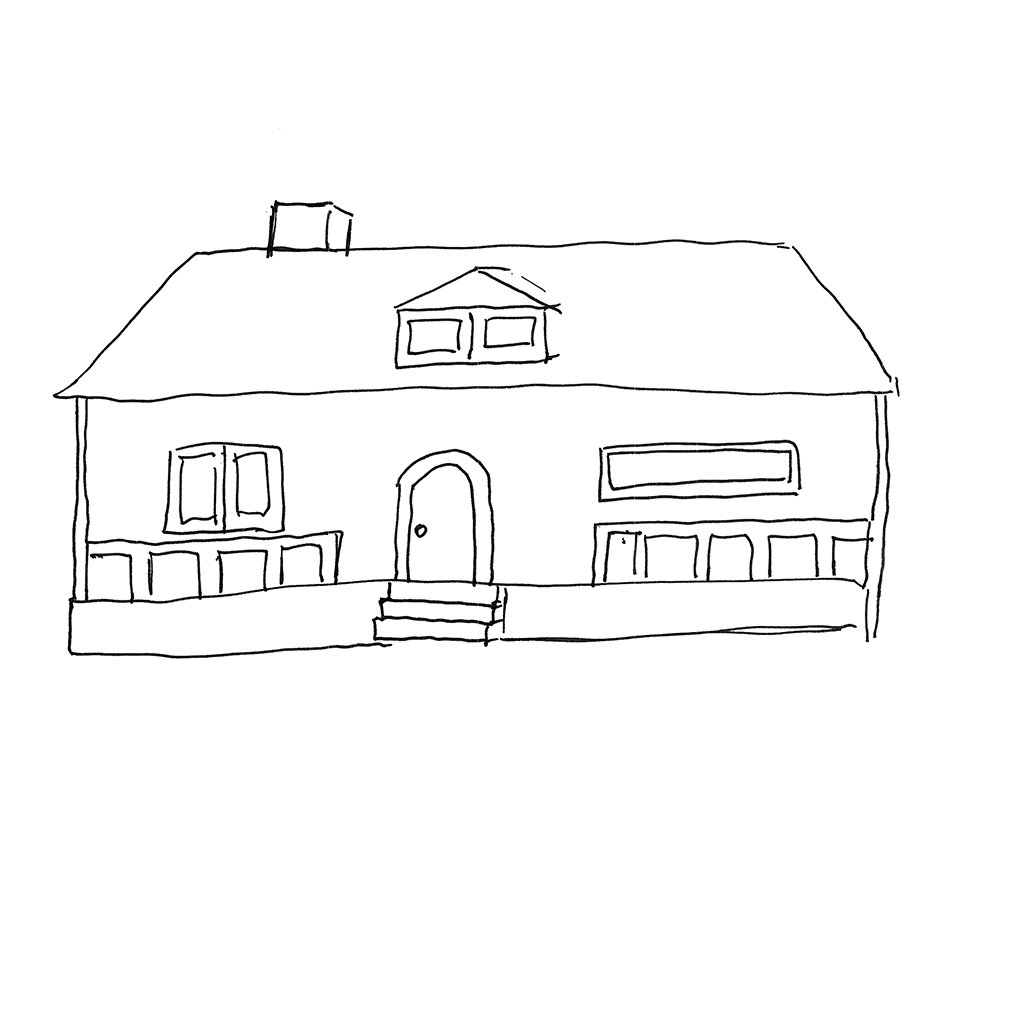
\includegraphics[width = 0.3\textwidth]{images/sketch2.jpg}}
\hspace{5mm}
\subfloat{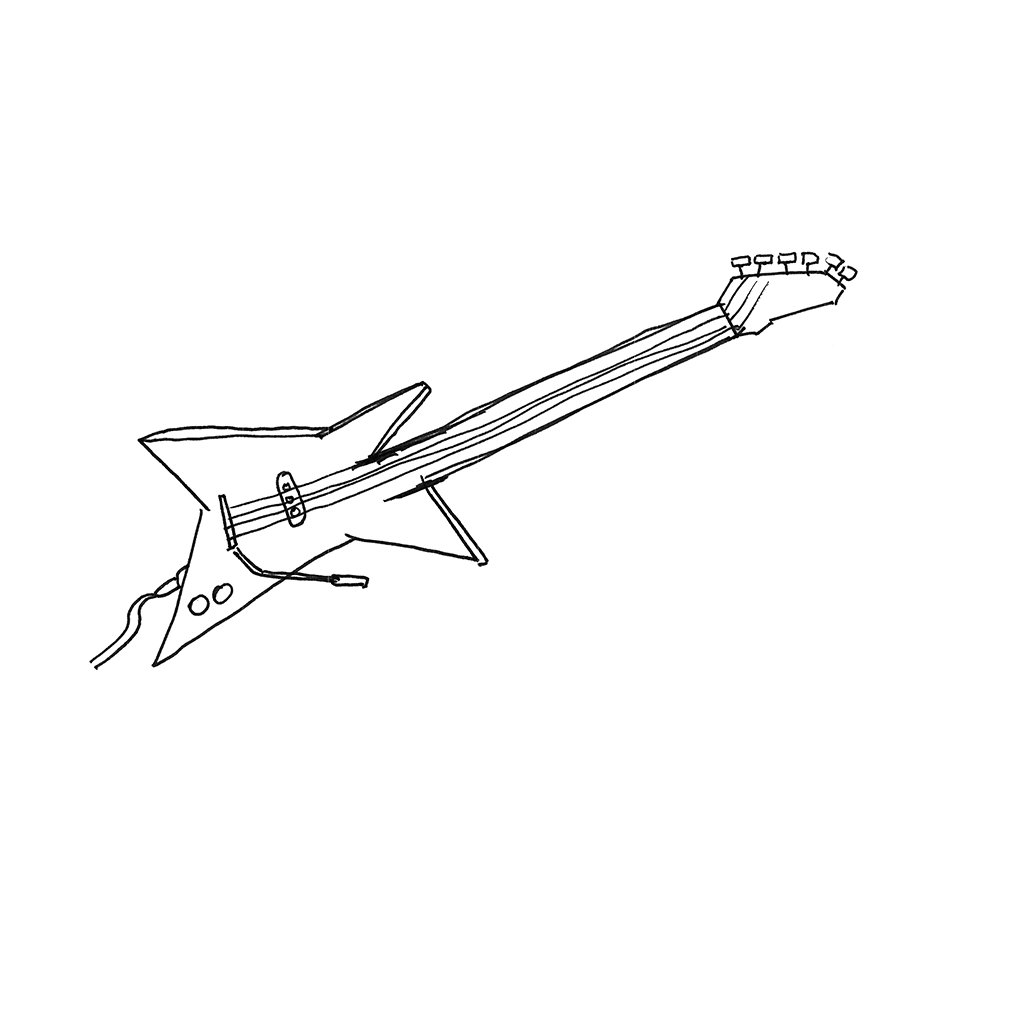
\includegraphics[width = 0.3\textwidth]{images/sketch3.jpg}}
\hspace{5mm}
\caption{example images from natural image and sketch training sets}
\label{fig:database_images}
\end{figure}

\section{Performance measurement}
Before we go further and present the experiments and results it is necessary to
introduce some additional terms. Such as metrics to measure their performance.

\paragraph{Mean squared error (MSE)} is an error measurement that
describes the error between an given or measured reference signal $\vec{x}$
and and the reconstruction(noisy approximation) $\vec{\tilde{x}}$ of it.
Mathematically it is defined as the average of the squared error between two
signals.
%The mean squared error is defined as:
\begin{equation*}
 MSE = \frac{1}{n} \sum_{i=0}^{n} \left( {\lVert x_i -
\tilde{x}_i\rVert^{2}}\right)
\end{equation*}
%We primarily use it for testing dictionary learning convergence and as a
%sub term for the measurement described in the next paragraph.

\paragraph{Peak signal-to-noise ration (PSNR)} describes the ratio between the
noise affecting a signal and the maximum possible signal amplitude. It is
expressed in a logarithmic decibel scale.
\begin{equation*}
 PSNR = 20 \cdot \log_{10} \left(\frac{MAX}{\sqrt{MSE}}\right)
\end{equation*}
Where $MAX$ is the maximum possible value of our signal. For an 8-bit
image it would be 255. For a 32-bit normalized image it would be 1. And $MSE$ is
the mean squared error between a reference signal and its reconstruction. The
PSNR is undefined for zero noise.

The PSNR is primarily used for comparison of the reconstruction quality of
lossy compression algorithms. Typical values for a lossy reconstruction lie in
a range between 30dB and
50dB.\footnote{\url{http://en.wikipedia.org/wiki/Peak_signal-to-noise_ratio}}
%e.g. relevant for de-noise

\paragraph{Bits per pixel (bpp)} 
For the comparison of compression ratio of images another well known practice is
to measure the required \emph{bits per pixel} short bpp. The bbp are calculated
by dividing the raw image data by the image's dimensions. For example an
uncompressed RGB color image with 8-bit of color depth requires 24-bits per
pixel, respectively a gray scale image with 8-bit for a single channel requires
8-bits. While compression algorithms are able to encode multiple pixels with few
coefficient leading to much lower bpp rates.
Looking at other well known compression algorithms such as JPEG or
JPEG 2000 a common ratio is about $\sim1.8$ bits-per-pixel for average
quality compression( JPEG quality of 50) of an natural image. 

\Todo{optinal: example image?, lower bit rates, Lewicki estimate for sparse
coding}

\paragraph{Test data}
In addition to the introduced metrics it is common practice to use some image
sets to compare test results of the different algorithms and parameter
configurations. As the dictionaries are specificaly trained for
reconstruction of the data in the training sets
(\prettyref{fig:database_images}) it is mandatory to also use
these image to test the reconstruction and
compression quality. 

In addition to this we want to know how good the dictionaries can reconstruct
and compress images outside of the database respectifly the training set. For
those comparisons we use a selection (\prettyref{fig:USC-SIPI}) from a
well known set of standard test images from the \emph{USC-SIPI Image
Database}\footnote{\url{http://sipi.usc.edu/database/}}
(\prettyref{fig:USC-SIPI}). 
%Including pictures such as Lena, Mandrill and Peppers.
\begin{figure}[H]
\centering
%\subfloat{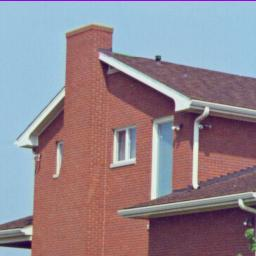
\includegraphics[width = 0.3\textwidth]{images/4_1_05.jpg}}
%\hspace{5mm}
\subfloat{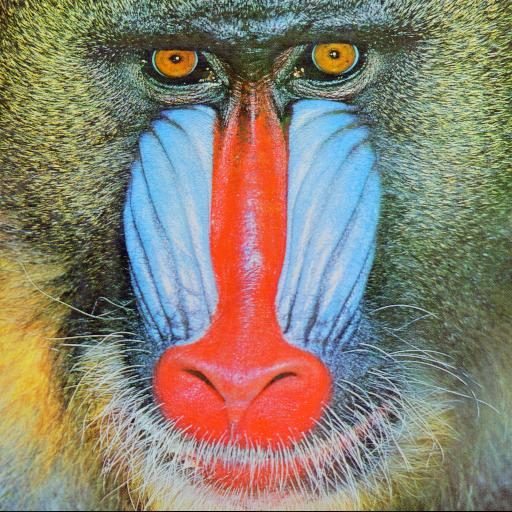
\includegraphics[width = 0.3\textwidth]{images/4_2_03.jpg}}
\hspace{5mm}
\subfloat{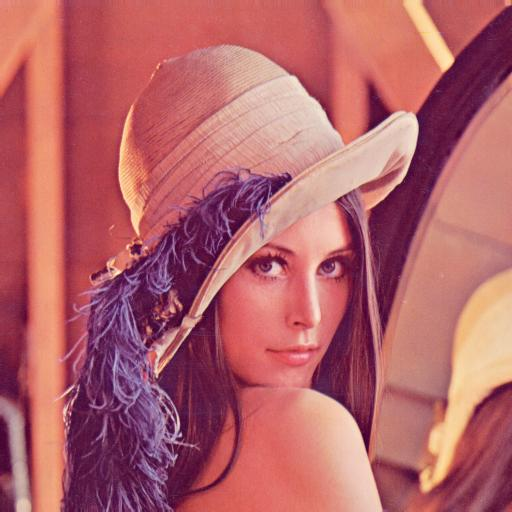
\includegraphics[width = 0.3\textwidth]{images/4_2_04.jpg}}
\hspace{5mm}
%\subfloat{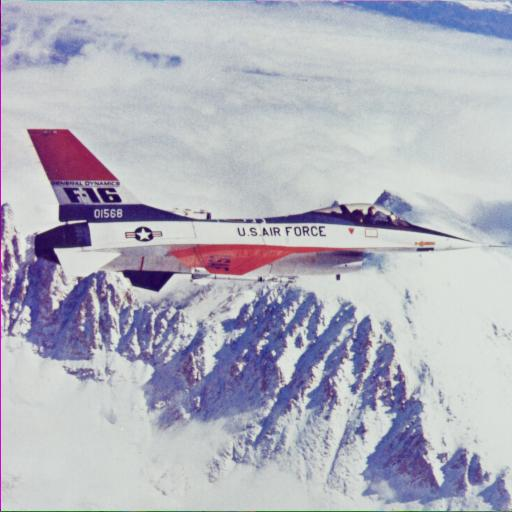
\includegraphics[width = 0.3\textwidth]{images/4_2_05.jpg}}
%\hspace{5mm}
%\subfloat{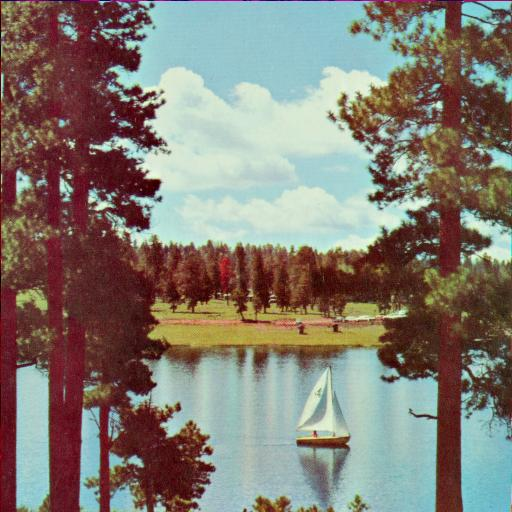
\includegraphics[width = 0.3\textwidth]{images/4_2_06.jpg}}
%\hspace{5mm}
\subfloat{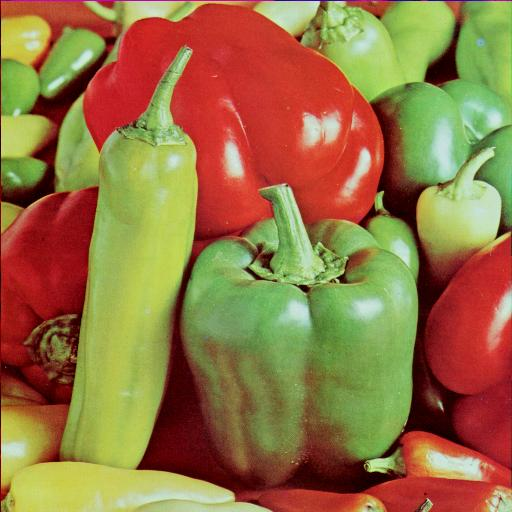
\includegraphics[width = 0.3\textwidth]{images/4_2_07.jpg}}
\caption{test images from USC-SIPI Image Database}
\label{fig:USC-SIPI}
\end{figure}

\section{Hardware setup} 
Computations were made on a cluster of 100 clients. Each 
configured with a AMD Athlon 64 X2 (2x2.6GHz) and 3GB RAM.
The operating system running Debian Linux with 32-bit kernel. 

\section{Learning parameters}
At first we needed to find good start settings for experiments with large set of
different samples and big dictionaries. This involves the
avarage number of learning coefficients, block size, sample selection strategy
and mini-batch size.

Mairal et al. already propose some learning parameters for their online
learning algorithm. But as most other they only learn dictionaries with
a small redundancy of up to four times and compact training sets with 100,000
to 1,000,000 samples that get randomly evaluated until convergence of the
dictionary.

We wanted to find start settings for experiments with large sets of
different samples with no reevaluation of the samples and dictionaries
with much bigger redundancy of 10 to 50 times.


\paragraph{Coefficents}
An average of 10 learning coefficients is suggested as it produces enougth
sparseness and leads to good and fast convergence of the dictionaries.
We tested if this also applies to big numbers of samples and bigger
dictionaries. We compared the reconstruction quality dependency on the average
number of coefficients in the learning process. Graphs show the avarage of a
set of test images from the training set. Both OMP (\prettyref{fig:coeffsOMP})
and LARS-Lasso (\prettyref{fig:coeffsLasso}) runs were made with the following
configuration.
\begin{table}[H]
%\caption{Configuration}
\centering
\begin{tabular}{| c | c | c |}
\hline
\multicolumn{3}{|c|}{configuration}\\
\hline
dict. size & block size & batch size \\
\hline
1000 & $8\times 8$ & 4000  \\
\hline
\end{tabular}
\end{table}

\begin{figure}[h]
\centering
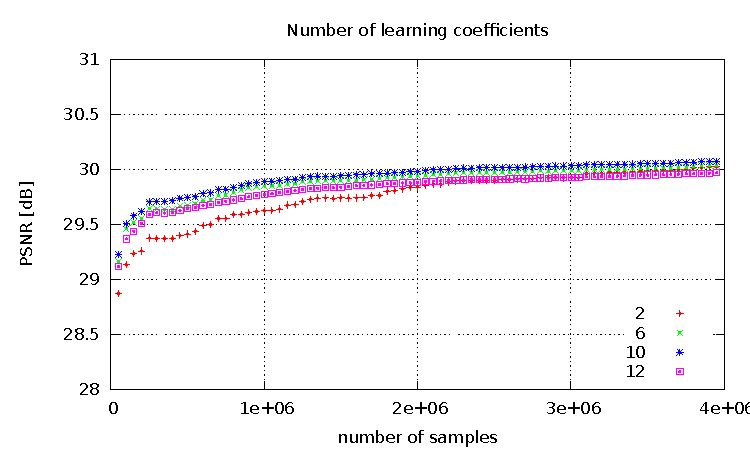
\includegraphics[width = 0.8\textwidth]{../tests/results/coeffsConverg.pdf}
\caption{reconstruction quality for different training coefficients (LARS)}
\label{fig:coeffsLasso}
\end{figure}

% \begin{figure}[h]
% \centering
% 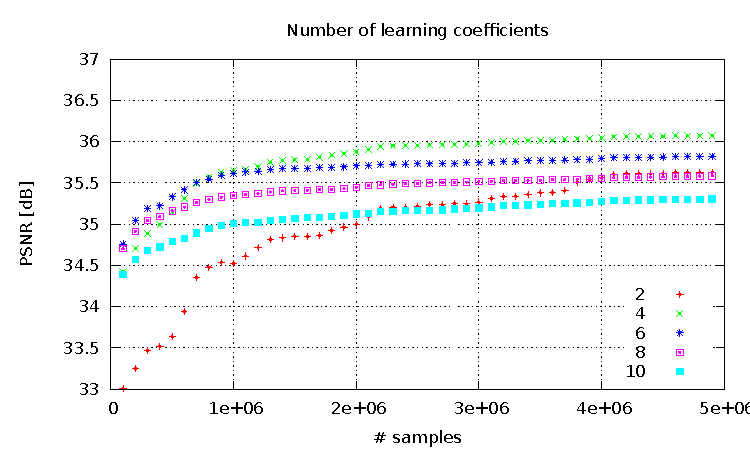
\includegraphics[width =
%0.8\textwidth]{../tests/results/old/coeffsConverg.pdf}
% \caption{reconstruction quality for different training coefficients (OMP)}
% \label{fig:coeffsOMP}
% \end{figure}



\begin{figure}[H]
\centering
\subfloat[2]{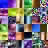
\includegraphics[width =
0.2\textwidth]{images/coeffsConvergOMP_0_1.jpg}}
\hspace{15mm}
\subfloat[10]{
\includegraphics[width =
0.2\textwidth]{images/coeffsConvergOMP_4_1.jpg}}
\caption{after 50,000 samples}
\label{fig:coeffsOMP50}
\end{figure}
\begin{figure}[H]
\centering
\subfloat[2]{
\includegraphics[width =
0.2\textwidth]{images/coeffsConvergOMP_0_2.jpg}}
\hspace{15mm}
\subfloat[10]{
\includegraphics[width =
0.2\textwidth]{images/coeffsConvergOMP_4_2.jpg}}
\caption{after 2,000,000 samples}
\label{fig:coeffsOMP2000}
\end{figure}

%Convergence of quality of different number of learning coefficients.
With high number of learning coefficents convergence is reached faster than
with a low number of coefficents but for large dicts fewer coefficents lead to
better reconstruction quality with larger training sets.

Allover we noticed that the LARS-Lasso produces dictionaries with better
reconstruction quality than the OMP. We concentrated our futher learning
experiments on the LARS-Lasso. 

\paragraph{Block size}
After the coefficents tests we compared the reconstruction quality dependency on
block size in the learning process of natural images. A LARS-Lasso run with
block sizes of $n=8,..,20$ were made. The dictionary size for each run was two
times the size of each signal $2m=2n^2$. And for the convergence test the
reconstruction coefficents were adjusted with an avarage of 8 coefficents for 64
pixels.

\begin{figure}[h]
\centering
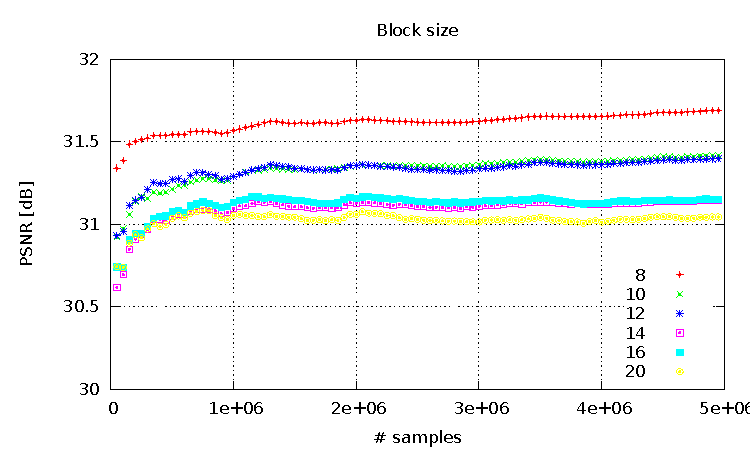
\includegraphics[width =
0.8\textwidth]{../tests/results/blockSizeConverg.pdf}
\caption{reconstruction quality for different block sizes}
\label{fig:dict size}
\end{figure}

Difference of quality of different block sizes.

The $8\times8$ block size has a significant better reconstruction quality. 
When we have a closer look at the structure of the atoms we will start to
understand why.

\paragraph{Structure}
Our training sets consists of JPEG images. 
%Do they resemble known structures from designed dictionaries? 
%How do these learned structures change with the block size of the atoms?
%What structure show samples from other groups of images?
Learn basis similar to DCT and wavelets/bandelets(time and freq locality) with
increasing block size.

For the natural images we tend to learn four major types of elements gradient,
checkerboard (low color more b/w), spot, edge.

\begin{figure}[h]
\centering
\subfloat{
\includegraphics[width = 0.3\textwidth]{images/gradient.png}}
\hspace{5mm}
\subfloat{
\includegraphics[width = 0.3\textwidth]{images/checkerboard.png}}
\hspace{5mm}
\subfloat{
\includegraphics[width = 0.3\textwidth]{images/spot.png}}
\hspace{5mm}
\subfloat{
\includegraphics[width = 0.3\textwidth]{images/edges.png}}
\hspace{5mm}
\subfloat{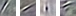
\includegraphics[width = 0.3\textwidth]{images/wavelet.png}}
\caption{common atoms}
\end{figure}

While looking at this we investigate some atoms of the sketch dictionary.

\paragraph{Mini-batch size}
For the small training sets Mairal et al. suggest mini-batch size of two to four
times the size of the the dictionary. No significant oberservations were made
and we stuck to these sizes. 

\newpage
\section{Dictionary size}
After we found good settings to learn from large sets of different images we
wanted to know how big we can make the dictionaries and still profit from them.
And if reconstruction quality increases with dictionaries size and when
convergence is reached. 

\begin{table}[H]
%\caption{Configuration}
\centering
\begin{tabular}{| c | c | c |}
\hline
\multicolumn{3}{|c|}{configuration}\\
\hline
coefficents & block size & batch size \\
\hline
10 & $8\times 8$ & 4000  \\
\hline
\end{tabular}
\end{table}

\begin{figure}[h]
\centering
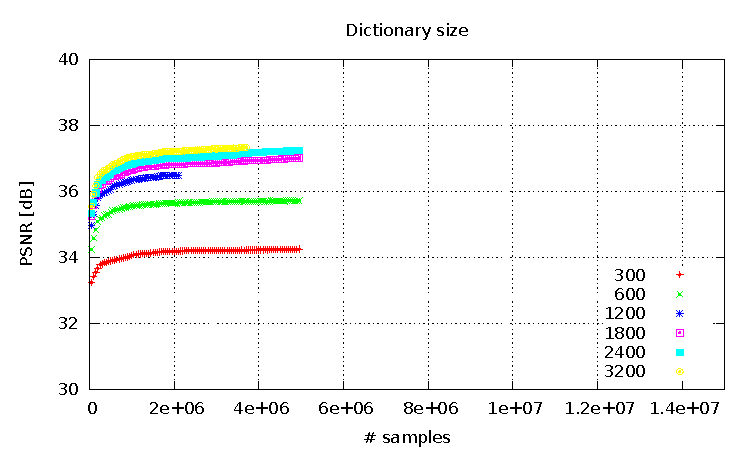
\includegraphics[width = 0.8\textwidth]{../tests/results/dictSizeOMP.pdf}
\caption{reconstruction quality for different dictionary sizes (OMP)}
\label{fig:dictSizeOMP}
\end{figure}

\begin{figure}[h]
\centering
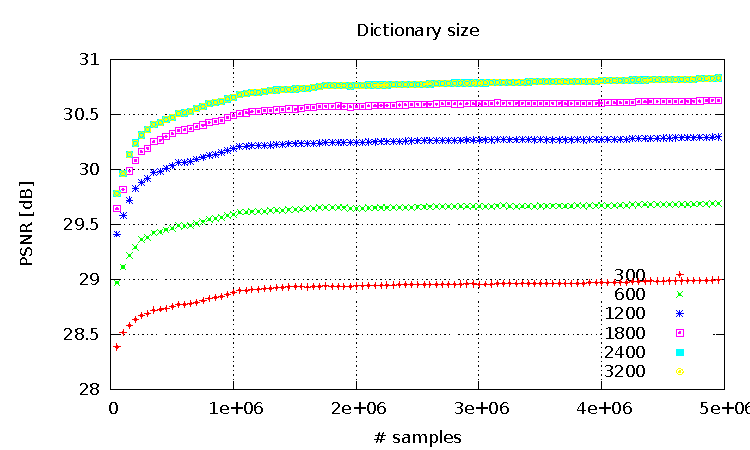
\includegraphics[width = 0.8\textwidth]{../tests/results/dictSizeLasso.pdf}
\caption{reconstruction quality for different dictionary sizes (Lasso)}
\label{fig:dict size}
\end{figure}

We see two things in this graphs. First convergence is almost reached
after 1,000,000 - 2,000,000 training samples. Second even this is a
logarithmical scale increasing dictionary size tends to a reach a maximum. The
problem is that big dictionaries do not learn enougth atoms leaving a lot of
them unused. This can be addressed with tweaks to the learning parameters like
increased number of learning coefficents. Or by replacing unused atoms with
elements from the training set. We tried a diffrent strategy and addresed this
issues with a the clustering approach from \prettyref{sec:clustering}.

\paragraph{Clustering}
In addition we compared the cluster approach performs in
comparisons to a dictionary learned in single. Each client in the cluster
learned a dictionary from batches of 1,000 images.
%based on the size of the training sets.

\begin{table}[h]
\centering
\begin{tabular}{| l | c | c |}
\hline\hline
Images & single & merged \\
\hline
inside & $34,29172 \pm 3,61$ & $35,04152 \pm 3,48$  \\
%outside & $35.5104 \pm 0.0$ & $35.5104 \pm 0.0$ \\
\hline
\end{tabular}
\caption{single vs. cluster}
\end{table}
The merged dictionary can reconstruct images with equal quality as the big
dictionary. But consists of multiple smaller dictionaries learned in clusters.


\newpage
\section{Compression}
Besides the ability of learned dictionaries 
we used the simple compression algorithm from \prettyref{sec:compression}.
and compared it to a collection of JPEG and JPEG 2000 compressed images with the
same file size. The objective was to investigate the compression ratio and if
the extra amount of index data is a big hit on the overall load.

One benefit of the learned dictionary approach that plays well in our
hands is the ability to to learn and use specific dictionaries for each group of
images. We tested this by learning a dictionary from a set of sketch images and
used it to compress sketches. A domain in which the JPEG compression performs
bad. As discovered before the natural images like block sizes of $8\times 8$
this is not necessarily true for the sketch images. They work fine with
$16\times 16$ blocks and enable us to reduce the amount of blocks.
\prettyref{fig:compressionDicts} shows the dictionaries. 


\begin{figure}[h]
\centering
\subfloat[natural images]{
\includegraphics[width =
0.5\textwidth]{images/natural_dict.jpg}}
\hspace{5mm}\label{fig:naturalDict}
\subfloat[sketches]{
\includegraphics[width =
0.5\textwidth]{images/sketch_dict.jpg}}\label{fig:sketchDict}
\caption{Dictionaries used for compression}
\label{fig:compressionDicts}
\end{figure}




% Difference in the selection strategy.
% Very noisy vs. smooth. 
% How this different selection strategies affect the learning step will be
% presented in the next section.
\subsection{Natural images}

\begin{figure}[h]
\centering
% \subfloat{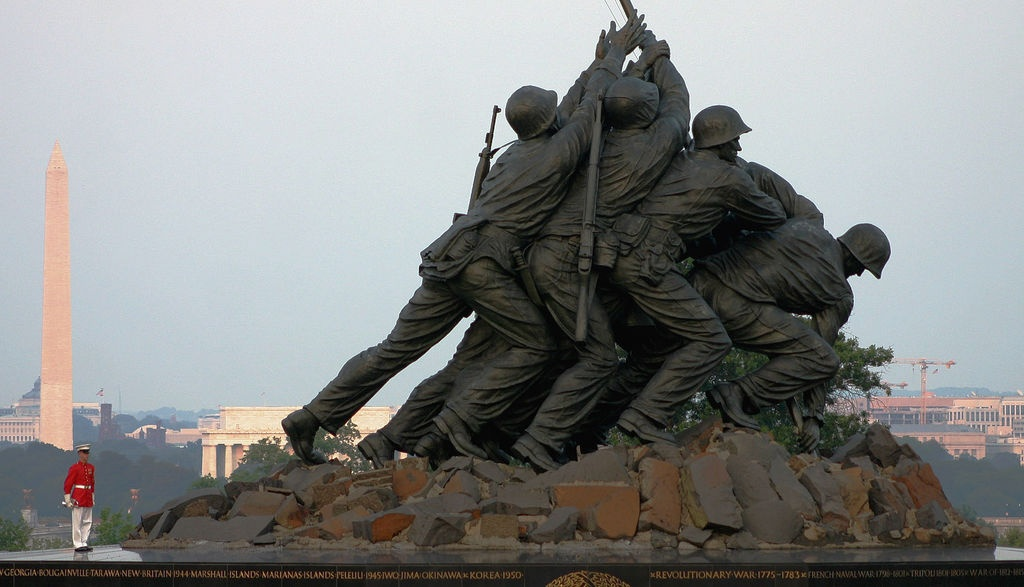
\includegraphics[width = 0.3\textwidth]{images/28979823.jpg}}
% \hspace{5mm}
% \subfloat{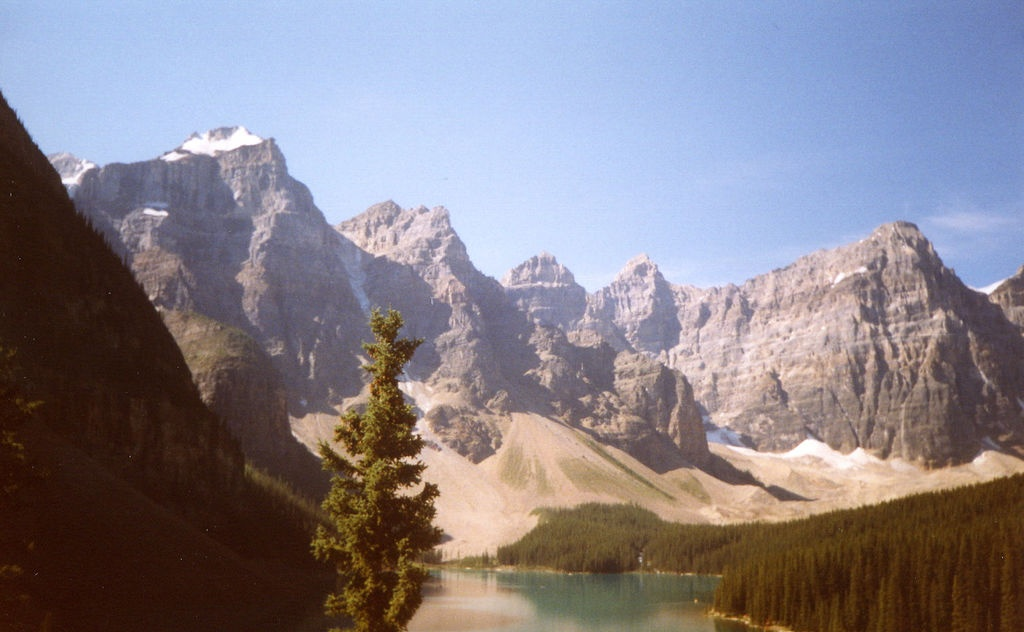
\includegraphics[width = 0.3\textwidth]{images/29018694.jpg}}
% \hspace{5mm}

\subfloat{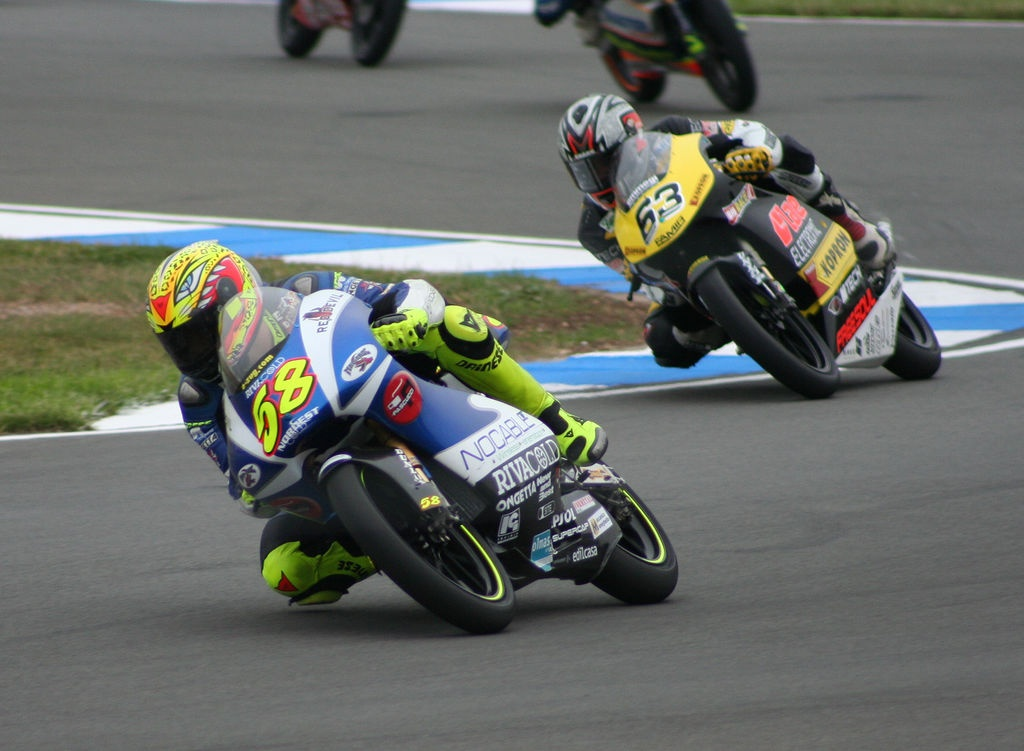
\includegraphics[width = 0.3\textwidth]{images/28803842.jpg}}
\hspace{5mm}
\subfloat{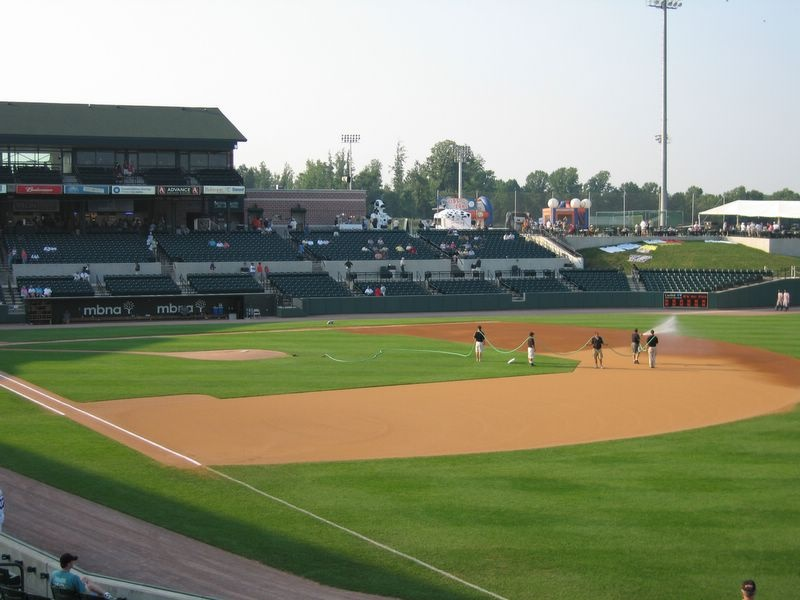
\includegraphics[width = 0.3\textwidth]{images/28894495.jpg}}
\hspace{5mm}
\subfloat{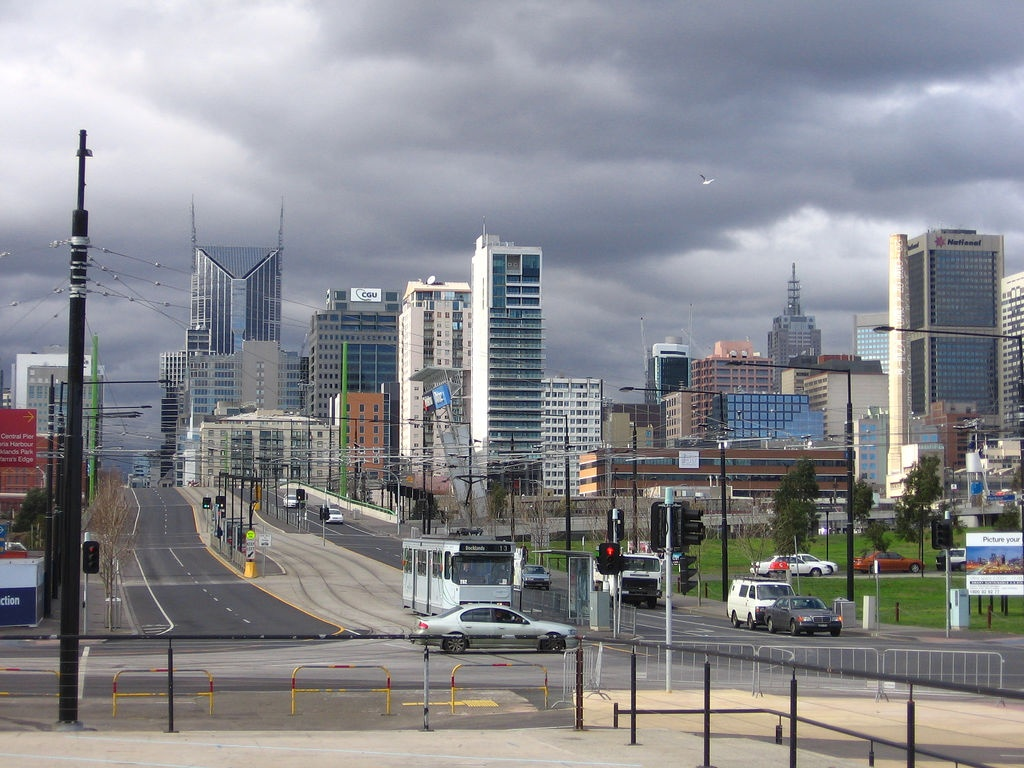
\includegraphics[width = 0.3\textwidth]{images/28952841.jpg}}
\hspace{5mm}
\subfloat{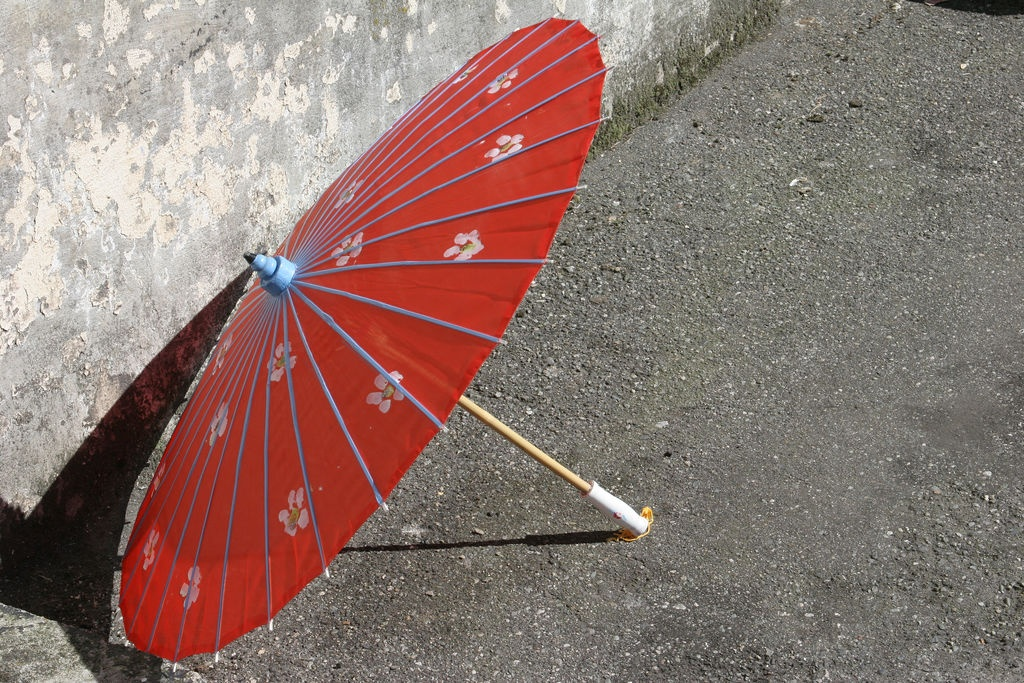
\includegraphics[width = 0.3\textwidth]{images/28874882.jpg}}
\caption{natural images}
%\label{fig:database_images}
\end{figure}

For the short time available the results show promising results. Compression of
natural images produces similar quality as the JPEG algorithm
\prettyref{tab:compression1} but does not reach the JPEG 2000 quality. 
Compression coding was done with the OMP as it turned out to work better with
the quantization step of our algorithm and requires less coefficents. 

\begin{table}[h]
%\caption{single vs. cluster}
\centering

\begin{tabular}{| l l | c | c | c|}
\hline\hline
Image & bpp & SPRS & JPEG & JPEG2000 \\
\hline
a & 1.12 & 31.2205 & 32.3289 & 36.6103 \\
b & 1.01 & 34.7735 & 35.0671 & 40.3299 \\
c & 1.8  & 29.0597 & 27.2556 & 31.7412 \\
d & 0.74  & 35.9499 & 35.5104 & 39.4195 \\
\hline
\end{tabular}
\caption{natural image compression results}
\label{tab:compression1}.
\end{table} 

\newpage
\subsection{Sketches}
The results get even better when looking at the sketch images
(\prettyref{fig:sketches}). Our algorithm can surpasses the JPEG compression
(\prettyref{tab:compression2}). \prettyref{fig:magnified} show some magnified
segments of image \ref{fig:sketch3} to ilustrate the reconstruction features.
There are less artifacts than in the JPEG images. The line segment atoms from
the dictionary show similarities to the wavelet based JPEG 2000 compression.

\begin{figure}[h]
\centering
\setcounter{subfigure}{0}
\subfloat[]{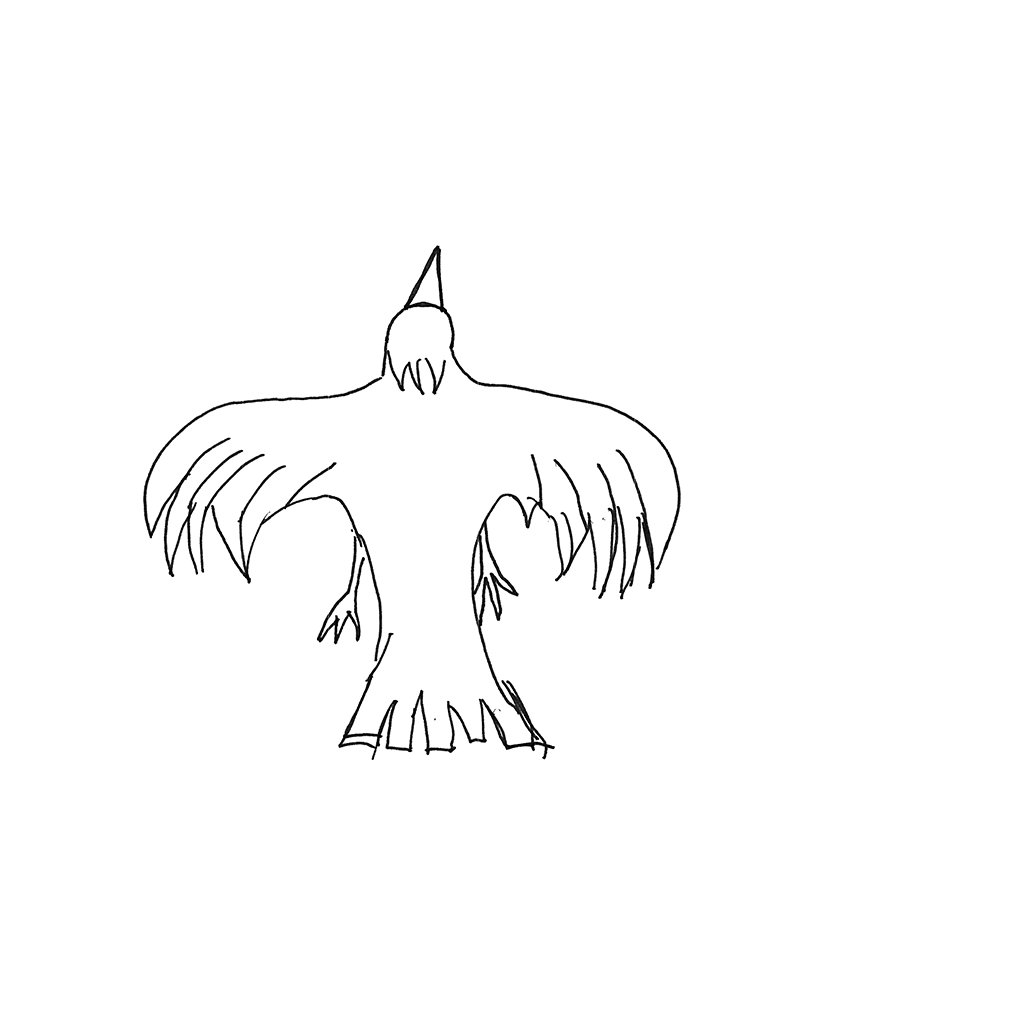
\includegraphics[width = 0.3\textwidth]{images/sketch1.jpg}}
\hspace{5mm}
\subfloat[]{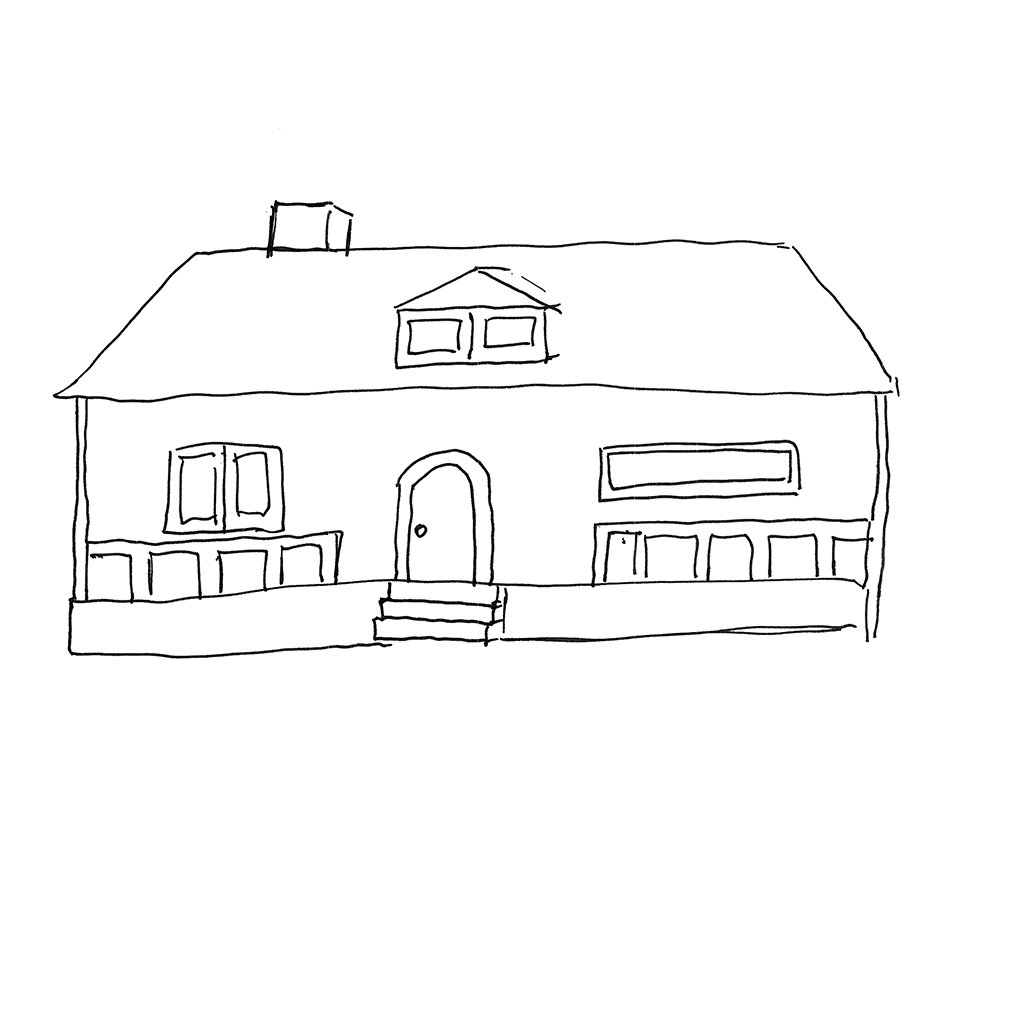
\includegraphics[width = 0.3\textwidth]{images/sketch2.jpg}}
\hspace{5mm}
\subfloat[]{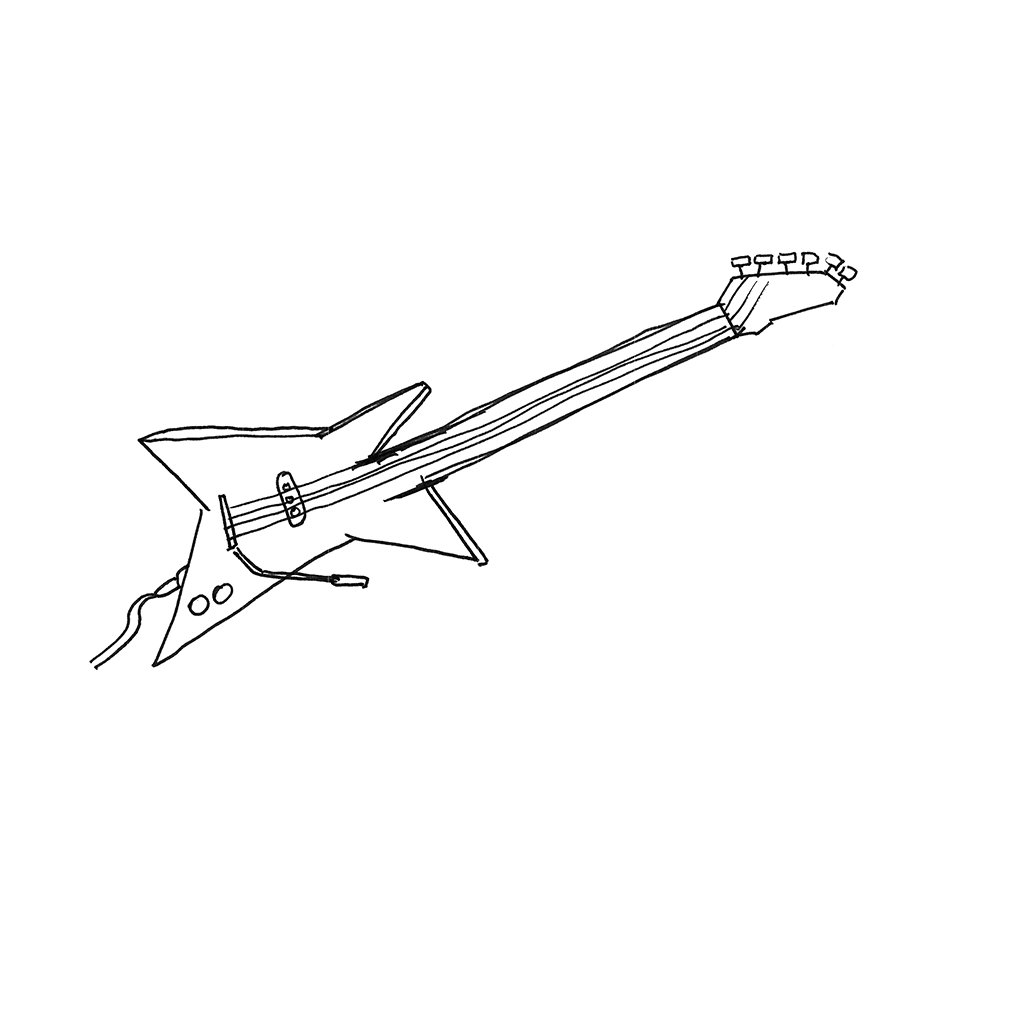
\includegraphics[width =
0.3\textwidth]{images/sketch3.jpg}\label{fig:sketch3}}
\hspace{5mm}
\caption{sketches}
\label{fig:sketches}
\end{figure}


\begin{table}[h]
%\caption{single vs. cluster}
\centering
\begin{tabular}{| c l | c | c | c|}
\hline\hline
Image & bpp & SPRS & JPEG & JPEG2000 \\
\hline
a & 0.084 & 33.9594 & 28.9578 & 38.3258  \\
b & 0.13 & 32.9002 & 34.5546 &  40.0159 \\
c & 0.08 & 32.5131 & 28.6558 & 36.3093  \\
\hline
\end{tabular}
\caption{sketch compression results}
\label{tab:compression2}
\end{table}

\begin{figure}[H]
\centering
\subfloat[original]{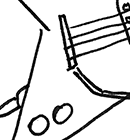
\includegraphics[width =
0.3\textwidth]{images/sketch_png.png}}
\hspace{5mm}
\subfloat[SPRS]{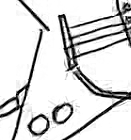
\includegraphics[width =
0.3\textwidth]{images/sketch_sprs.png}}
\hspace{25mm}
\subfloat[JPEG]{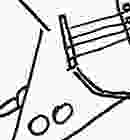
\includegraphics[width =
0.3\textwidth]{images/sketch_jpeg.png}}
\hspace{5mm}
\subfloat[JPEG2000]{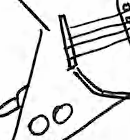
\includegraphics[width =
0.3\textwidth]{images/sketch_2000.png}}
\caption{}
\label{fig:magnified}
\end{figure}


% This chapter shows the results and discussion for the following experiments.
% % Reconstruction quality is mean of PSNR of images inside and outside of
% % the training sets.
% \begin{enumerate}
%  \item Convergence of reconstruction quality for different dictionary sizes.
%  \item Comparison of reconstruction quality of dictionaries
% in single and in cluster runs. 
%  \item Comparison of compression quality between learned dictionaries, JPEG
%and
% JPEG2000  on natural images and sketches.
%  \item Observations of structures of dictionary atoms from different
% groups of images and block sizes.
% \end{enumerate}









